\documentclass[a0paper,fleqn]{betterportraitposter}

% PACKAGES
\usepackage[none]{hyphenat}
\usepackage{lipsum}

%%%% Uncomment the following commands to customise the format

%% Setting the height of the top and bottom (colored) bars
%% Uncomment either of the following lines it you want to change the defaults heights of the top or bottom bars.
% \setlength{\mainfindingheight}{0.5\paperheight} % Top bar
% \setlength{\bottomboxheight}{0.10\paperheight} % Bottom bar

%% Setting the page margin

%% Changing font sizes
% Text font
%\renewcommand{\fontsizestandard}{\fontsize{28}{35} \selectfont}
% Main column font
%\renewcommand{\fontsizemain}{\fontsize{28}{35} \selectfont}
% Title font
%\renewcommand{\fontsizetitle}{\fontsize{28}{35} \selectfont}
% Author font
%\renewcommand{\fontsizeauthor}{\fontsize{28}{35} \selectfont}
% Institution font
%\renewcommand{\fontsizeauthor}{\fontsize{28}{35} \selectfont}
% Section font
%\renewcommand{\fontsizesection}{\fontsize{28}{35} \selectfont}

%% Changing font sizes for a specific text segment
% Place the text inside brackets:
% {\fontsize{28}{35} \selectfont Your text goes here}

%% Changing colours
% Background of main claim box (options include: imperialblue, empirical, theory, methods and intervention
% Default is empirical
% \renewcommand{\maincolumnbackgroundcolor}{intervention}

% Font on main and bottom boxes
% \renewcommand{\maincolumnfontcolor}{empirical}

% You can add a custom RGB color like so (example here is University of Glagow blue):
\definecolor{UoGBurgundy}{RGB}{125, 35, 57}
\renewcommand{\maincolumnbackgroundcolor}{UoGBurgundy}




\begin{document}	

%% Top box with main message
\mainfinding{\textbf{Main finding} goes here, translated into \textbf{plain English}. \textbf{Emphasize} the important words.}


%% Title, author and affiliations section
\titlebox{
    \title{The Very Long and Technical Title of Your Super Interesting Study Which Will Save the World}  
    
    \author{Mike Morrison, Rafael Bailo and Daniel Bradford}
    
    \institution{Optional Institution Under Name}
    }
% End of title stuff
    
    
%% Central box with traditional content
\centerbox{\begin{multicols}{3}
\section{Introduction}
Here is an itemised list:
\begin{itemize}
\item The first item.
\item The second item.
\item The third item.
\end{itemize}

\section{Fundamental Theorem of Calculus}
If $f$ is continuous on the closed interval $[a,b]$ and $F$ is the indefinite integral of $f$ on $[a,b]$, then
\begin{equation}
\int_a^b f(x)\,\mathrm{d}x = F(b)-F(a).
\end{equation}

\section{Conclusion}
This is a great poster format!
\columnbreak

Here you can add \textbf{supplementary material}. For instance, a new diagram:
\begin{center}
% Commutative diagram with edges passing under/over
% Author: Stefan Kottwitz, http://texblog.net/
% Retrieved from: http://www.texample.net/tikz/examples/commutative-diagram/
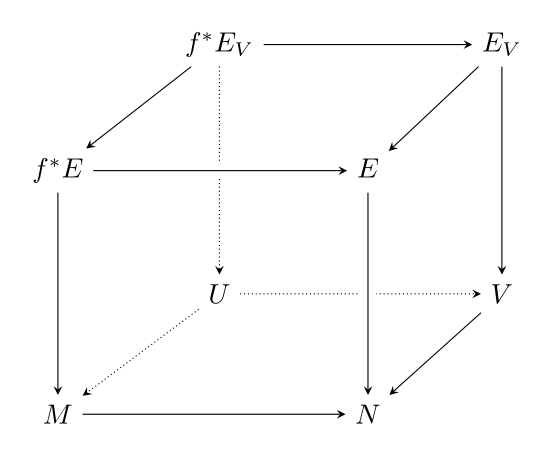
\includegraphics[width=\columnwidth]{img/tikzexample2}
\end{center}
\columnbreak
Some cute ducklings:
\begin{center}
% Picture of ducklings
% Author: Magda Ehlers, https://www.pexels.com/@magda-ehlers-pexels
% Retrieved from: https://www.pexels.com/photo/selective-focus-photo-of-flock-of-ducklings-perching-on-gray-concrete-pavement-1300355/
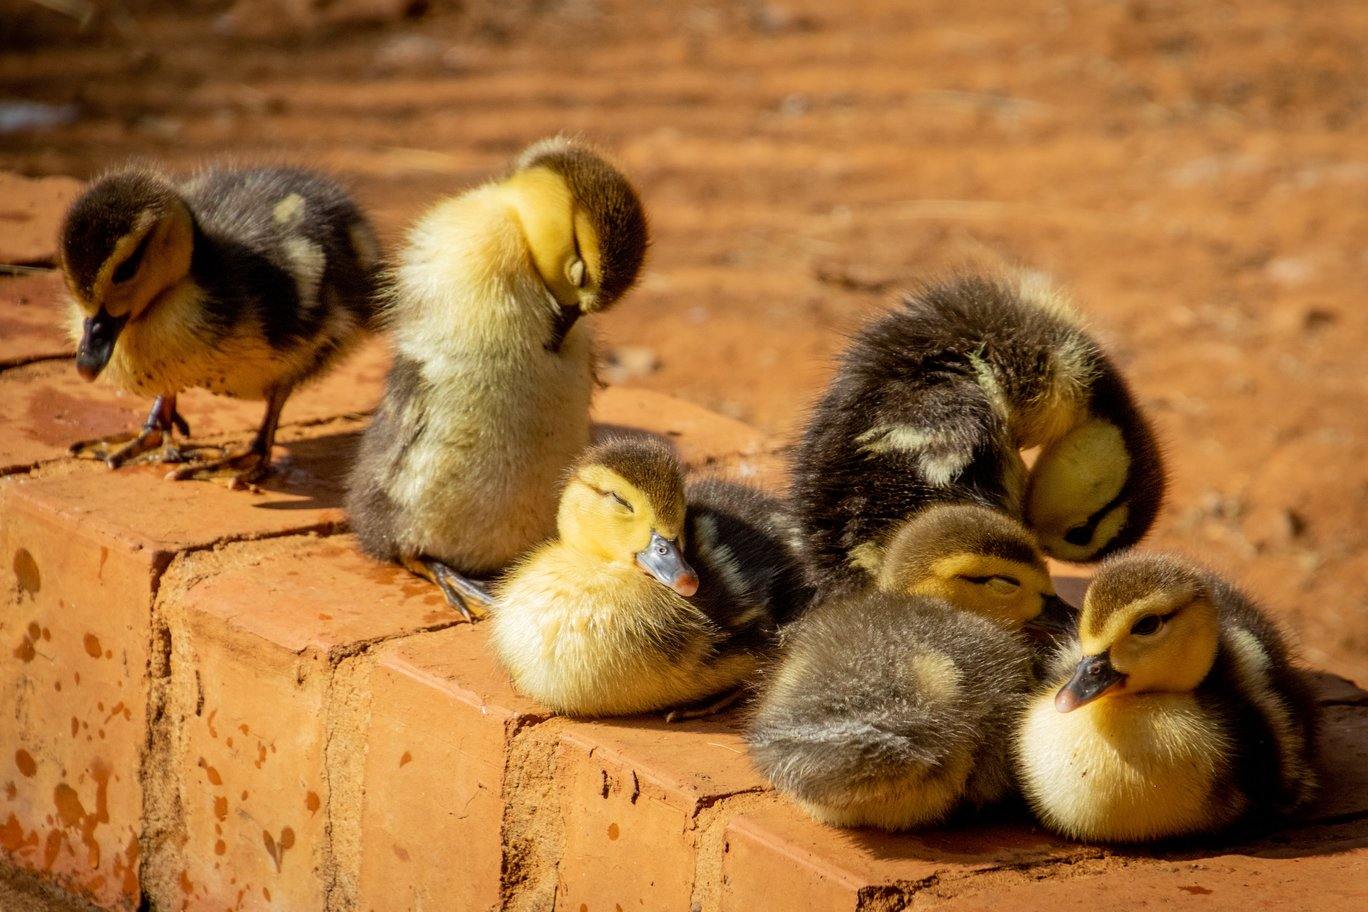
\includegraphics[width=\columnwidth]{img/ducklings}
\end{center}


\end{multicols}

}
% End of central box



% Bottom box with QR code
\bottombox{
    %% QR code
    \qrcode{img/qrcode}{img/smartphoneWhite}{Scan QR code to get the full paper}
    % Comment out the line below out to hide logo
    \hfill\bottomboxlogo{img/logo.eps} % \hfill shifts the logo across so it meets the right hand side margin
    % Note that \bottomboxlogo takes an optional width argument. It defaults to the following: 
    % \hfill\bottomboxlogo[width=\textwidth]{<path_to_image_file>} 
    % where \textwidth is actually the width of a minipage which is defined in the \bottombox command of
    % betterportaitposter.cls It's a standard \includegraphics command in there, so easy to change if 
    % you need to add a border etc.
    
}
% End of bottom box


%\qrcode{img/qrcode}{img/smartphoneWhite}{
%\textbf{Take a picture} to
%\\download the full paper
%}


%% Compact QR code (comment the previous command and uncomment this one to switch)
%\compactqrcode{img/qrcode}{
%\textbf{Take a picture} to
%\\download the full paper
%}

%}

\end{document}